\thispagestyle{empty} 
\vspace*{1cm}
\sffamily
\begin{flushright}
	B.Sc. thesis\\
	Bachelor of Science in Software Development
\end{flushright}
\vspace{0.9cm}
\begin{figure}[ht]
 	\centering
    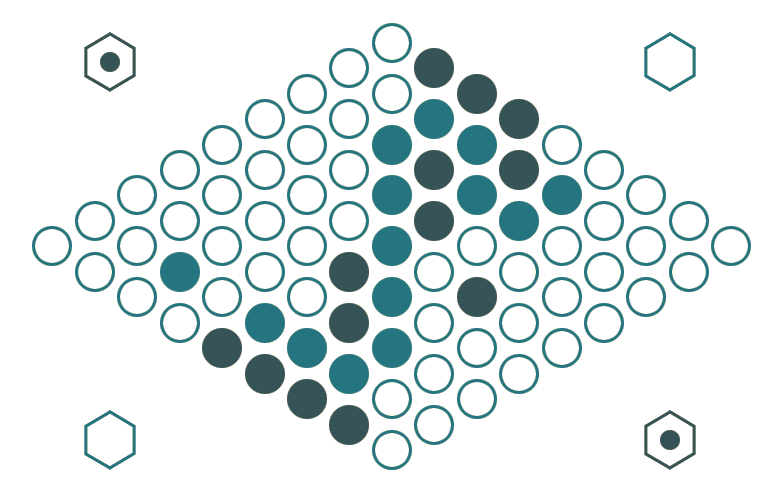
\includegraphics[scale=0.45]{graphics/capture4.png}
    \makeatletter
\end{figure}
%\vspace{0.0cm}
%\begin{hyphenrules}{nohyphenation}
%	\HUGE{Playing Hex with Deep Reinforcement Learning and Tree Search %on Consumer Grade Hardware}\par
%\end{hyphenrules}
\vspace{0.9cm}
%\begin{hyphenrules}{nohyphenation}
	\linespread{1.2}\huge{Generality of Deep Reinforcement Learning for Playing Abstract Strategy Games}\par
	\vspace{0.1cm}
	\linespread{1.2}\LARGE{Playing Hex with Neural Networks and Tree Search on Consumer Grade Hardware}\par
%\end{hyphenrules}

\vspace{0.9cm}
\large{Magnus Malthe Jacobsen (mjac@itu.dk)}
\vspace{0.9cm}

\normalsize{Copenhagen, 2019}
\begin{figure}[ht]
    
\includegraphics[width=0.7\textwidth]{graphics/ITU_logo_UK.jpg}
    \caption*{}
    \makeatletter
\end{figure}

